\section{面向对象设计}

\subsection{设计说明}
面向对象设计部分从参与者边界、核心对象、活动控制、交互时序、对象协作、状态演化、软件构成和运行部署八个层面描述系统。各类图围绕同一组核心概念展开，包括场景建模师、行业分析师、系统管理员、项目、场景版本、任务、结构化命令、插件作业、执行结果以及日志与仿真对象。通过统一角色命名、任务边界和结果承接对象，不同图件能够共同刻画系统从输入到执行、从结果生成到版本留存的完整设计。

\subsection{用例图}
图\ref{fig:oo_usecase} 展示了系统对外提供的主要能力及其角色边界。场景建模师通过登录认证进入建模工作区，可执行项目管理、场景建模、布局调整、智能修改和结果导出等操作；行业分析师进入分析工作区后执行结果分析与结果导出；系统管理员进入治理工作区后执行权限配置、日志审计和服务监控。图中还明确了智能修改与草图解析、任务确认、插件执行之间的包含关系，以及结果分析与结果导出之间的扩展关系。

从功能划分上看，建模工作区对应系统的生产链路，分析工作区对应系统的结果消费链路，治理工作区对应系统的运行维护链路，三者以登录认证作为统一入口，并在系统边界内形成相互独立但共享数据成果的能力分区。场景建模师能够直接触发场景生成、布局调整和智能修改，因此其用例最靠近任务执行与场景版本生成；行业分析师不直接参与生成，而是建立在既有版本和仿真结果之上完成观察、比较和导出；系统管理员则不处理具体业务结果，而是保障权限、服务和审计环境的稳定运行。

该图在设计层面说明了两个关键问题。其一，系统采用按角色分区、按工作台组织能力的外部交互方式，不同角色的可见能力集合并不相同。其二，智能修改并不是孤立能力，而是以内含的草图解析、任务确认和插件执行为处理链路，因此其实现上必然关联自然语言解析、约束检查和插件调度三个内部机制。

\begin{figure}[!htbp]
\centering
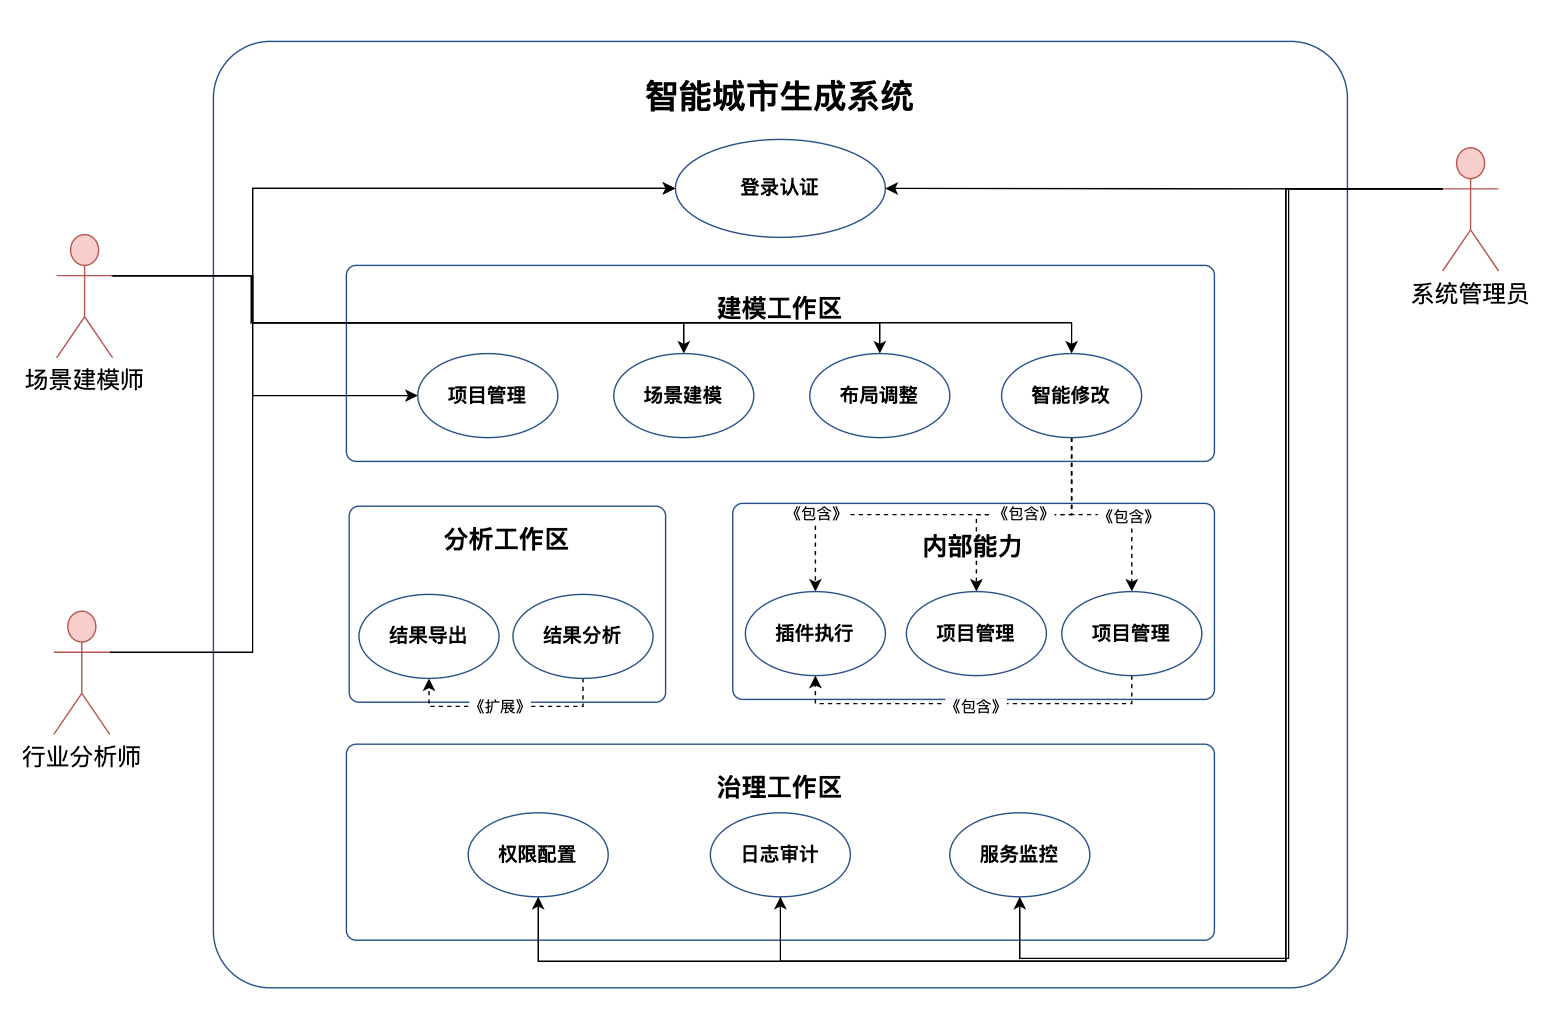
\includegraphics[width=\textwidth]{figures/01.png}
\caption{系统用例图}
\label{fig:oo_usecase}
\end{figure}

\subsection{类图}
图~\ref{fig:oo_class} 对系统静态结构进行了对象化展开，整体按身份与权限、项目与场景、任务与执行、仿真与治理四个对象域组织。身份与权限域由 \texttt{User}、\texttt{Role}、\texttt{Permission} 和 \texttt{Session} 组成，用于表达用户、角色、权限和会话之间的约束关系；项目与场景域由 \texttt{Project}、\texttt{SceneVersion}、\texttt{SceneObject}、\texttt{LayoutModel} 和 \texttt{Asset} 组成，用于表达项目聚合场景版本、场景版本承接布局与对象的组织方式；任务与执行域由 \texttt{TaskInput}、\texttt{ParseResult}、\texttt{StructuredCommand}、\texttt{Task}、\texttt{PluginJob} 和 \texttt{ExecutionResult} 组成，用于表达从输入规范化到任务执行结果回传的处理链路；仿真与治理域由 \texttt{SimulationPlan}、\texttt{DynamicObject} 和 \texttt{OperationLog} 组成，用于表达仿真结果和审计记录的承接关系。

在对象关系上，\texttt{Project} 聚合多个 \texttt{SceneVersion}，说明同一项目下允许保留多轮生成与修改结果；\texttt{SceneVersion} 聚合场景对象和布局模型，说明版本不仅保存最终对象集合，也保存其空间组织依据；\texttt{TaskInput} 与 \texttt{ParseResult}、\texttt{StructuredCommand}、\texttt{Task} 之间形成从输入理解到可执行命令的转换链；\texttt{Task} 进一步关联 \texttt{PluginJob} 和 \texttt{ExecutionResult}，说明系统内部将任务管理与插件执行结果显式区分；\texttt{SimulationPlan} 关联多个 \texttt{DynamicObject}，说明仿真方案负责承接动态交通、人群和船只等可观察对象；\texttt{OperationLog} 与用户和任务形成引用关系，说明关键操作和执行状态需要保留可追溯记录。

该图在设计上提供了三个静态基础。第一，项目、版本、任务和执行结果形成了系统的主数据骨架，使不同章节中的活动图、顺序图和状态图都可以围绕同一对象域展开。第二，解析结果与结构化命令的独立存在，说明 LLM 输出不会直接落到几何生成层，而是必须先转化为可验证、可调度的中间对象。第三，仿真对象、日志对象与核心任务对象并列存在，说明系统不仅关注生成，还同时关注结果分析与治理留痕。

\begin{figure}[!htbp]
\centering
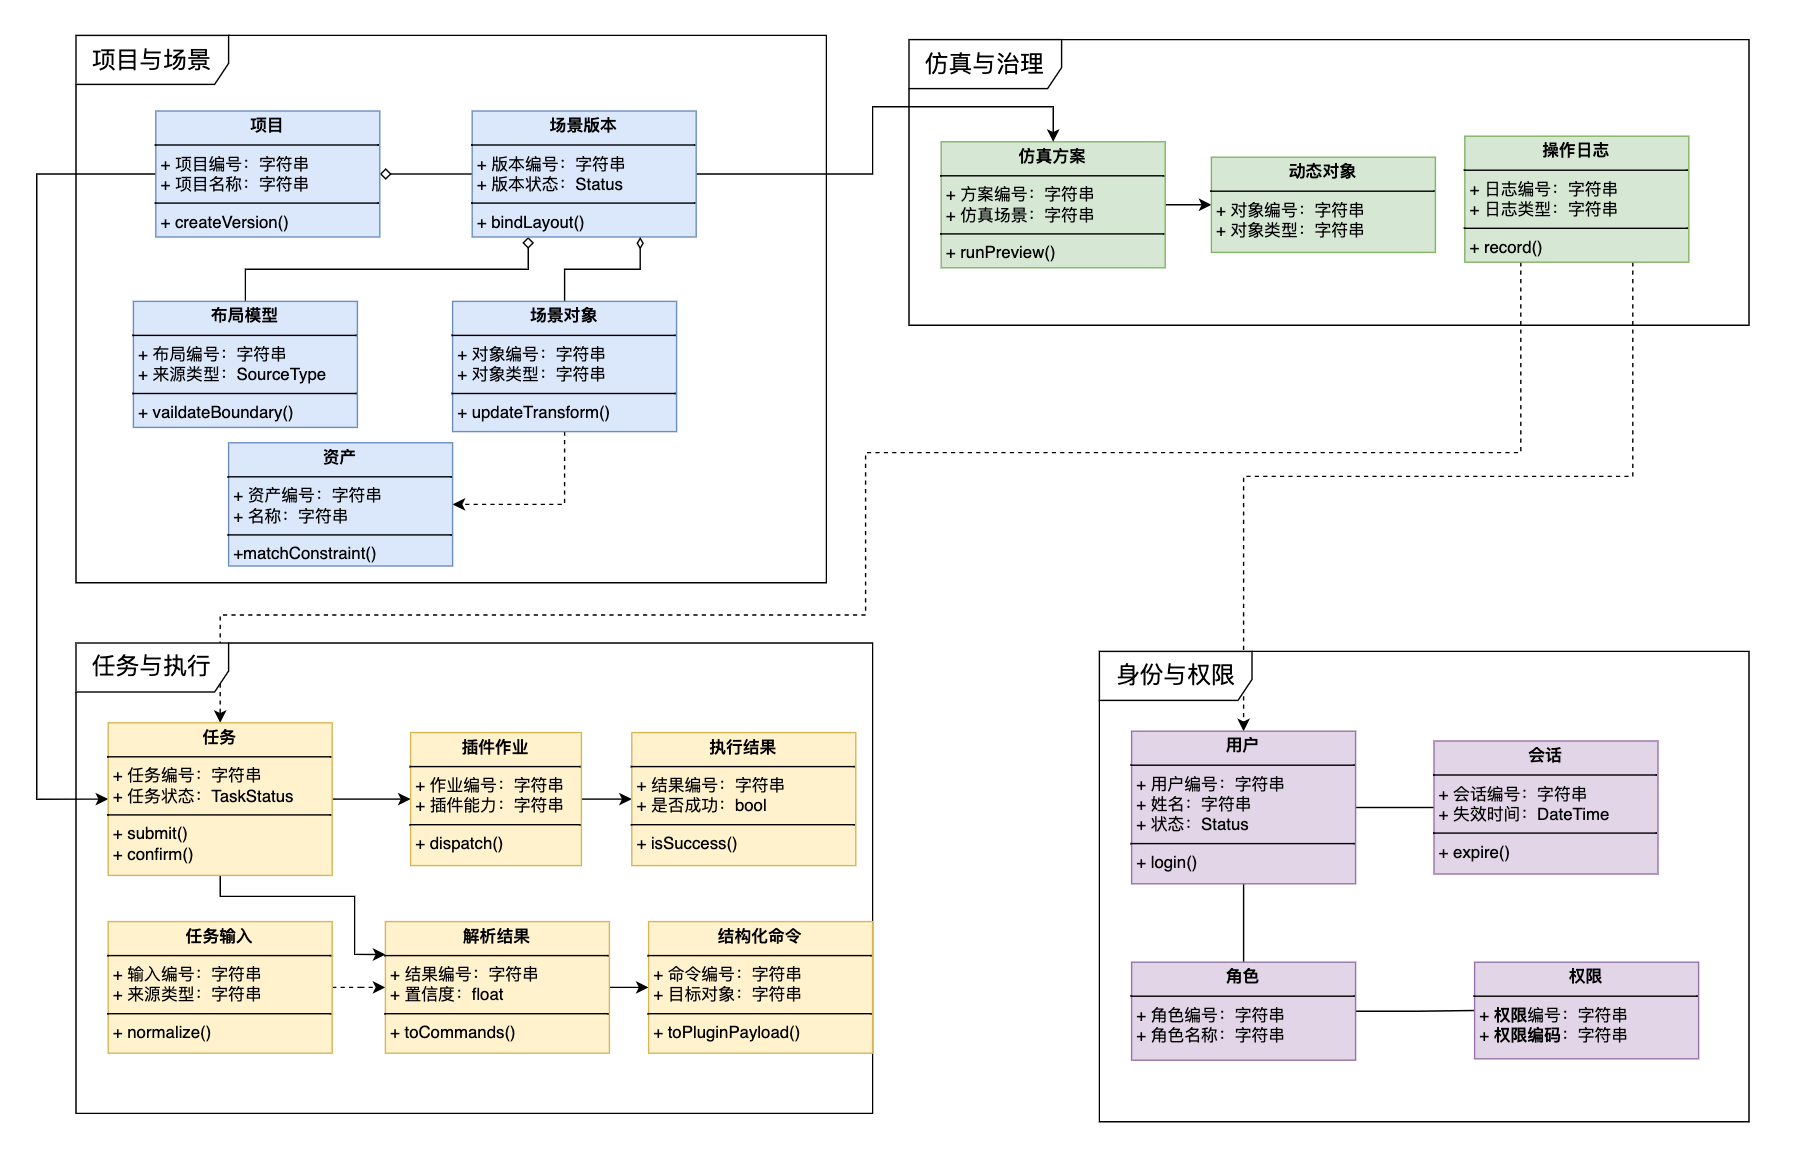
\includegraphics[width=\textwidth]{figures/02.png}
\caption{系统核心类图}
\label{fig:oo_class}
\end{figure}

\subsection{活动图}
活动图用于描述系统在控制流层面的组织方式。图~\ref{fig:oo_activity_main} 给出核心生成流程，图~\ref{fig:oo_activity_modeler}、图~\ref{fig:oo_activity_analyst} 和图~\ref{fig:oo_activity_admin} 分别补充三类角色在各自工作台中的活动路径。主活动图强调统一执行闭环，角色活动图强调不同用户在同一系统中的操作边界和回退路径。

\subsubsection*{1. 核心生成活动图}
核心生成活动图见图~\ref{fig:oo_activity_main}。流程从输入接收开始，依次经过场景上下文读取、意图解析、执行条件校验、任务确认、插件执行、版本保存和结果回看等环节。若当前输入无法直接执行，则流程返回补充信息和重新解析；若插件执行失败，则系统返回错误并允许重新提交；若结果仍需继续修改，则流程回到新的输入轮次。该图表达了系统以任务确认为界、以插件执行为核心、以版本回写和结果回看构成闭环的控制方式。

该图中的四个泳道分别对应场景建模师、主系统、LLM 解析模块和 Blender 插件，体现了控制权在不同处理阶段的转移方式。建模师负责提出意图和确认任务，主系统负责组织上下文、校验条件和登记状态，LLM 解析模块负责将输入转化为结构化任务建议，Blender 插件负责执行几何生成、替换或布局调整。这种泳道划分避免了将所有动作混写在单一流程中，使系统在控制层、解释层和执行层之间的职责边界更加清晰。

从控制逻辑上看，该图包含两个重要判定节点。第一个判定节点是“是否满足执行条件”，用于表达资源缺失、约束冲突或解析歧义时，流程必须回退到补充信息和重新解析，而不能直接进入执行。第二个判定节点是“执行是否成功”，用于表达插件执行后的失败重提与成功回写分流。结合最后的“是否继续修改”判断，该图完整刻画了系统从一次输入到多轮迭代的闭环机制。

\begin{figure}[!htbp]
\centering
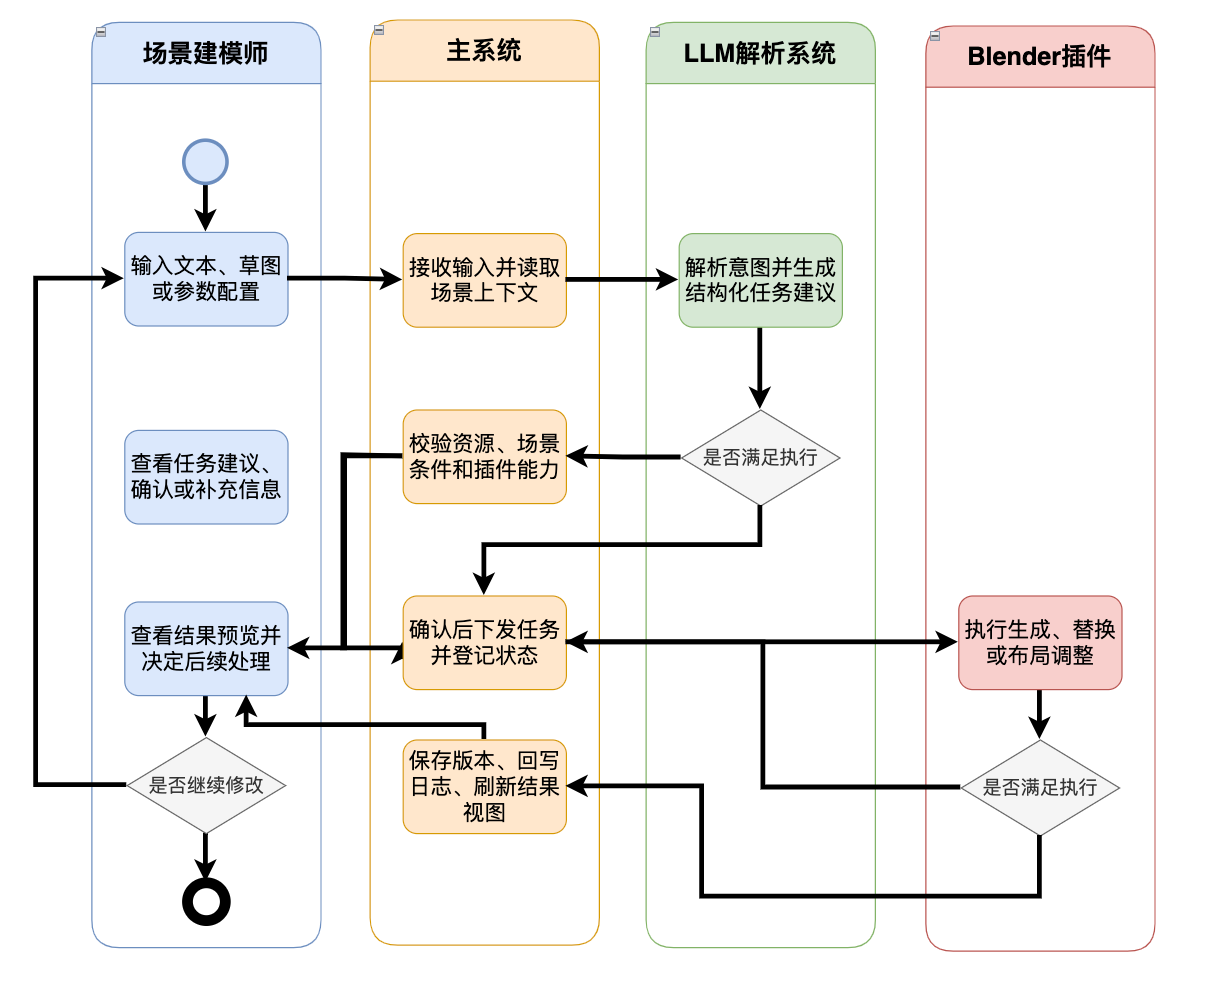
\includegraphics[width=\textwidth]{figures/04.png}
\caption{核心生成活动图}
\label{fig:oo_activity_main}
\end{figure}

\subsubsection*{2. 角色活动图}
图~\ref{fig:oo_activity_modeler} 进一步细化了场景建模师在建模工作台中的活动路径，覆盖项目选择、输入提交、任务确认、结果观察、版本保存与继续修改等环节，体现了多轮生成与局部修正过程。该图与主活动图相比，更强调建模师在版本创建、结果判断和局部重生成中的操作位置。

图中从“登录并进入建模工作台”开始，分化出“选择项目、创建版本或加载既有场景”和“输入文本、草图、点线集或参数配置”两条准备路径，随后在“查看解析后的任务建议并确认、补充或调整参数”处汇合，说明建模任务既依赖已有项目上下文，也依赖本轮输入内容。后续“观察生成结果与动态预览”以及“保存版本、导出场景或继续局部修改”构成结果处理阶段，其中判定节点“结果是否满足预期”决定流程是结束于版本保存，还是返回前部继续迭代。

该图支撑的设计重点在于说明建模师并非一次性提交后被动等待，而是持续参与项目版本组织、任务解释确认和结果质量判断三个环节。也就是说，系统中的智能建模并不是全自动批处理，而是一个带有人工确认和多轮反馈的交互式生产流程。

\begin{figure}[!htbp]
\centering
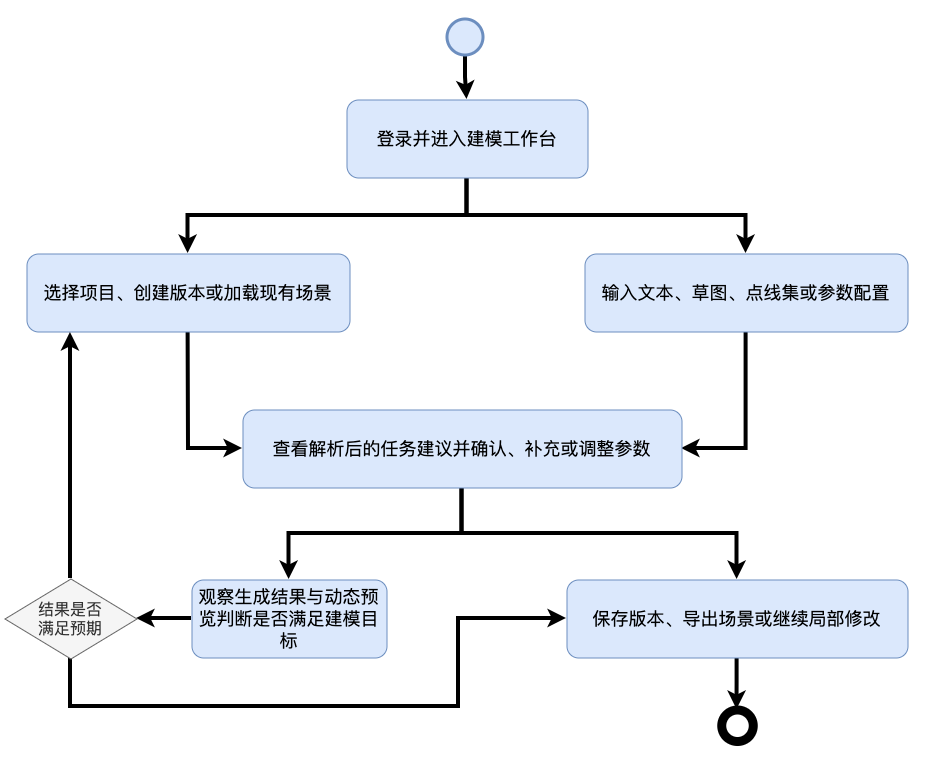
\includegraphics[width=0.9\textwidth]{figures/041.png}
\caption{场景建模师活动图}
\label{fig:oo_activity_modeler}
\end{figure}

行业分析师活动图对应图~\ref{fig:oo_activity_analyst}，其主线围绕分析对象选择、静态结果查看、仿真回放、方案比较和结果导出展开。该图反映了分析工作台以结果消费、仿真观察和多方案比较为主的处理链路。

图中先由分析师选择项目、方案或场景版本，确定待分析对象，再进入静态结果查看与关键指标查看阶段；之后通过“运行或回放仿真结果”观察车辆、人群、船只等动态差异，并在“比较不同方案并形成阶段性分析判断”节点形成分析结论。若仍需继续比较，则返回上游继续观察其他方案；若比较完成，则导出截图、结果文件或分析报告。

该图表明分析工作台并不承担生成职责，而是依赖已有版本和仿真结果开展消费、比较和判断工作。因此系统在这一角色下更强调结果可视化、指标一致性、对比链路和导出能力，而不是任务编排或插件执行能力。

\begin{figure}[!htbp]
\centering
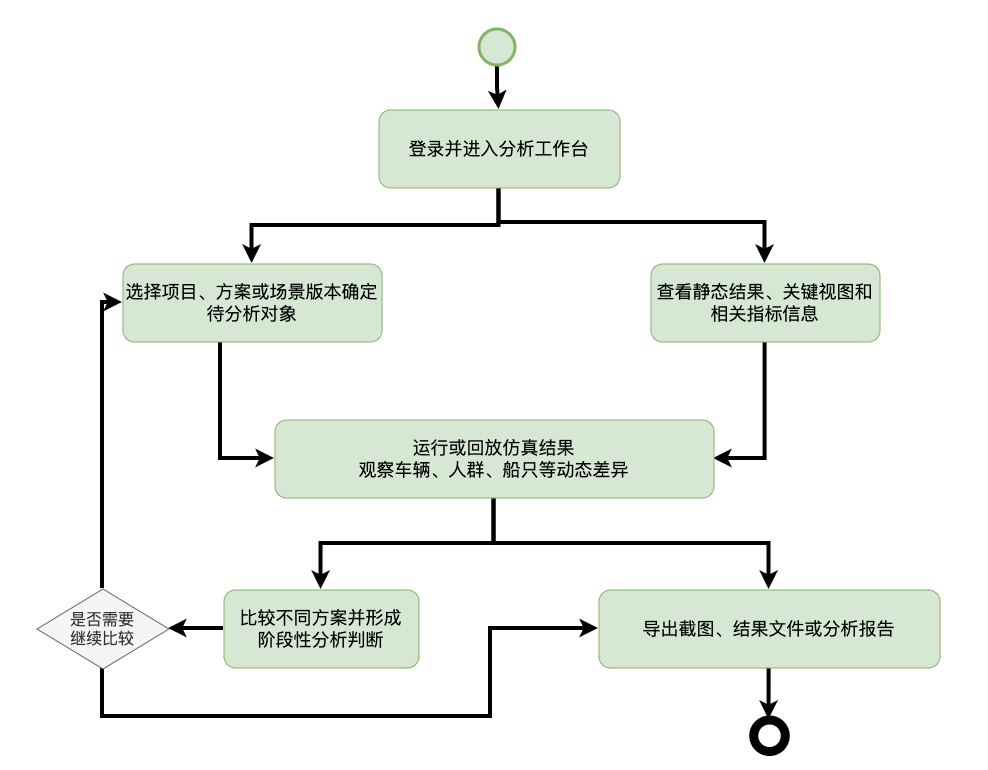
\includegraphics[width=0.9\textwidth]{figures/043.png}
\caption{行业分析师活动图}
\label{fig:oo_activity_analyst}
\end{figure}

系统管理员活动图如图~\ref{fig:oo_activity_admin}，围绕用户与权限维护、服务配置、任务监控、异常处理和审计留痕展开。该图表达了治理工作台以配置管理、运行监控和异常闭环处理为核心的维护过程。

图中从后台管理工作台进入后，分别展开为“维护用户、角色和权限关系”和“配置插件、模型服务和资源库接入状态”两类基础治理动作，随后汇合到“监控任务执行状态、查询日志并定位权限或服务异常”这一监控节点。若发现越权、失败任务或资源失效，则进入异常处理；若处理后仍存在持续异常，则流程回到上游继续巡检，否则通过“保存配置变更并形成审计记录”完成当前治理闭环。

该图所强调的不是业务产出，而是系统可用性和可追溯性。它说明管理员工作台必须同时支撑权限管理、服务接入、运行监控、异常处置和审计留痕五类能力，从而为建模和分析流程提供稳定的运行环境。

\begin{figure}[!htbp]
\centering
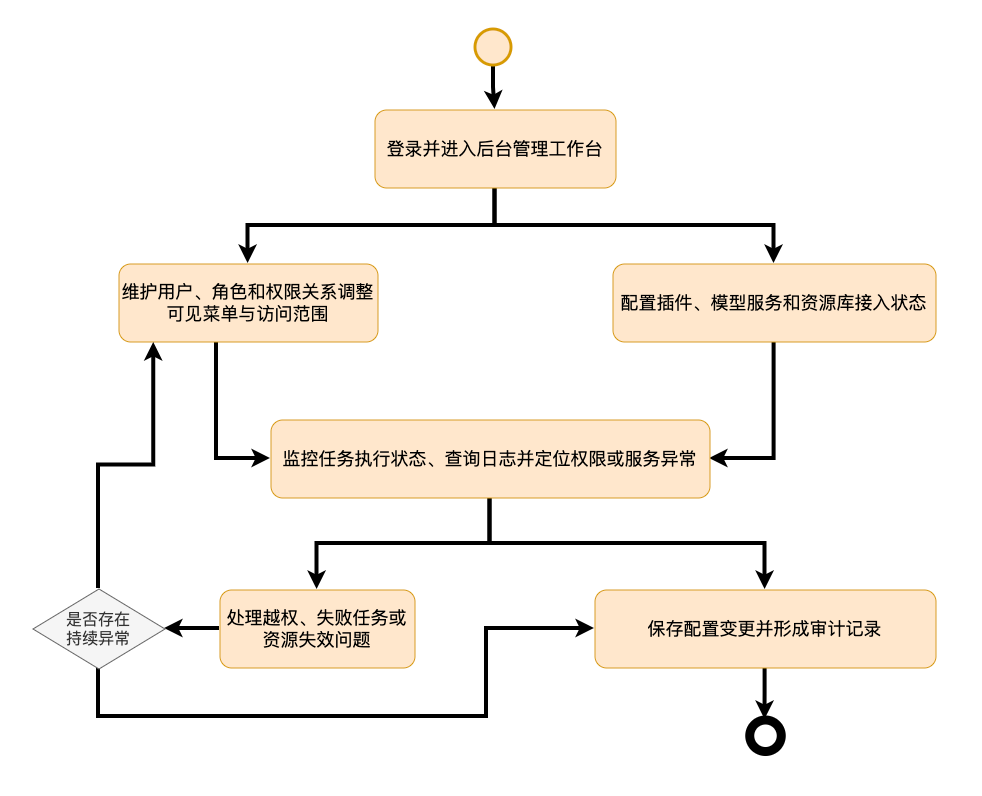
\includegraphics[width=0.9\textwidth]{figures/042.png}
\caption{系统管理员活动图}
\label{fig:oo_activity_admin}
\end{figure}

\subsection{顺序图}
顺序图~\ref{fig:oo_sequence} 按时间先后描述了一次建模任务的主要交互过程。建模师经由主系统提交输入后，任务编排模块先创建草稿并从项目存储读取上下文快照，再调用解析执行服务生成任务计划，并将任务解释返回界面。若当前信息不足，用户补充输入后重新进入解析；若任务可直接执行，则由用户确认后提交正式任务。随后，任务编排模块调用解析执行服务执行任务，在执行期间持续回传进度并更新界面状态，执行结束后完成版本保存和结果展示。

从参与对象上看，该图包含建模师、主系统、任务编排、解析执行服务和项目存储五个生命线。主系统负责接收输入并向编排层转交，任务编排负责承接草稿、组织上下文和控制后续流程，解析执行服务负责完成解析与执行，项目存储负责提供场景快照并保存最终结果。通过这种生命线划分，图中将“谁负责组织流程”和“谁负责执行业务”区别开来。

从消息序列上看，该图可以分为三个阶段。第一阶段是草稿创建与上下文读取，对应从 \texttt{submitInput()} 到 \texttt{loadContext()} 的调用链；第二阶段是任务解释与用户确认，对应 \texttt{parseIntent()}、\texttt{explainTask()}、\texttt{refineInput()} 和 \texttt{confirm()} 的交互；第三阶段是正式执行与结果回传，对应 \texttt{submitTask()}、\texttt{executeTask()}、\texttt{progress()}、\texttt{saveVersion()} 和 \texttt{showResult()}。该图明确了系统在时序上的职责分配和状态推进逻辑。

\begin{figure}[!htbp]
\centering
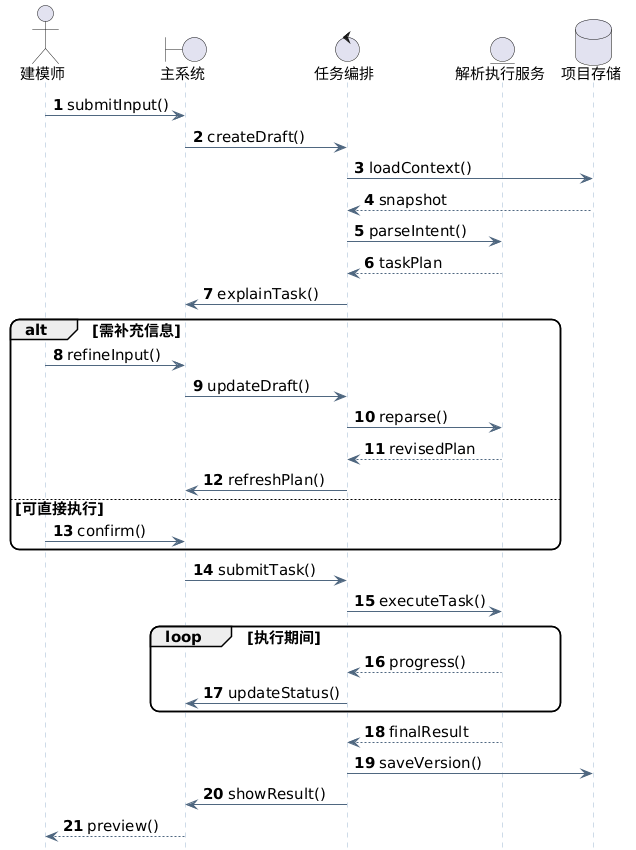
\includegraphics[width=\textwidth]{../UML_Project_Detailed_Fixed/03_SequenceDiagram.png}
\caption{场景任务顺序图}
\label{fig:oo_sequence}
\end{figure}

\subsection{协作图}
图~\ref{fig:oo_collaboration} 从对象协作角度展开了一次任务提交和执行过程，涉及建模工作台、任务编排器、资源上下文服务、LLM 解析服务、约束检查器、插件适配器、Blender 插件、版本管理器和仿真预览服务。任务编排器负责承接输入、读取上下文、调用解析和约束检查并返回任务解释；确认后，插件适配器负责下发插件作业，版本管理器负责生成新版本并请求仿真预览服务刷新结果。

与顺序图相比，该图更强调“哪些对象发生连接”和“消息如何在对象之间分发”。图中的任务编排器位于协作中心，一方面向资源上下文服务和 LLM 解析服务请求解释支持，另一方面向约束检查器获取告警和可执行性信息；确认后，消息通过插件适配器传递到 Blender 插件，再由版本管理器负责结果固化和面板刷新。仿真预览服务并不直接参与生成，而是在版本产生后提供可观察结果。

该图揭示了系统在对象协作层面的结构特点，即输入理解、约束校验、插件执行、版本管理和仿真预览并不是串成一个单体模块，而是通过一组相对独立的对象协同完成。这样的设计有利于后续替换解析服务、扩展插件能力或增补新的预览服务。

\begin{figure}[!htbp]
\centering
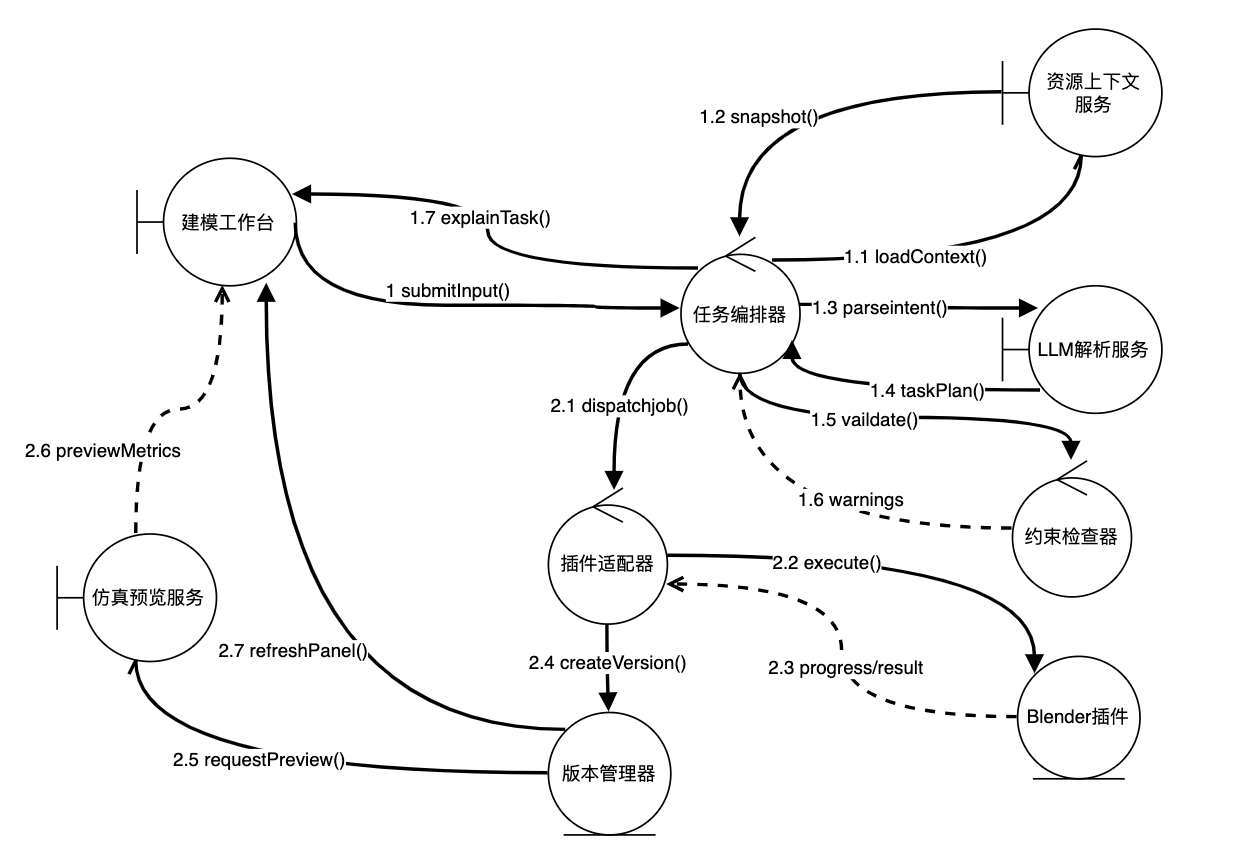
\includegraphics[width=\textwidth]{figures/05.png}
\caption{任务协作图}
\label{fig:oo_collaboration}
\end{figure}

\subsection{状态图}
状态图~\ref{fig:oo_state} 以 \texttt{Task} 为核心对象，描述任务从创建到归档的生命周期。任务创建后先处于草稿状态，提交解析后进入解析中；若存在歧义或条件缺失，则转入待补充，补充完成后重新解析；若生成结构化任务，则进入待确认；确认后进入排队中和执行中；执行成功后进入结果检查，再根据处理结果转入归档或回到草稿继续编辑；若解析或执行失败，则转入失败状态，并根据后续操作重新编辑或归档失败记录。

该图中的状态转换可以归纳为四个阶段。第一阶段是任务形成阶段，包括草稿、解析中和待补充，重点解决输入是否足以形成可执行任务的问题；第二阶段是任务确认阶段，由待确认状态承担，重点解决用户是否接受系统解释的问题；第三阶段是任务执行阶段，包括排队中和执行中，重点解决插件资源调度和执行反馈的问题；第四阶段是结果处理阶段，包括结果检查、失败、已取消和已归档，重点解决结果采纳、异常留痕和生命周期结束的问题。

状态图在设计上的意义在于将“任务是否存在”进一步细化为“任务当前处于何种处理位置”。这样一来，界面层可以基于状态决定允许的操作，调度层可以基于状态决定后续处理逻辑，日志层也可以基于状态变化形成清晰的审计轨迹。

\begin{figure}[!htbp]
\centering
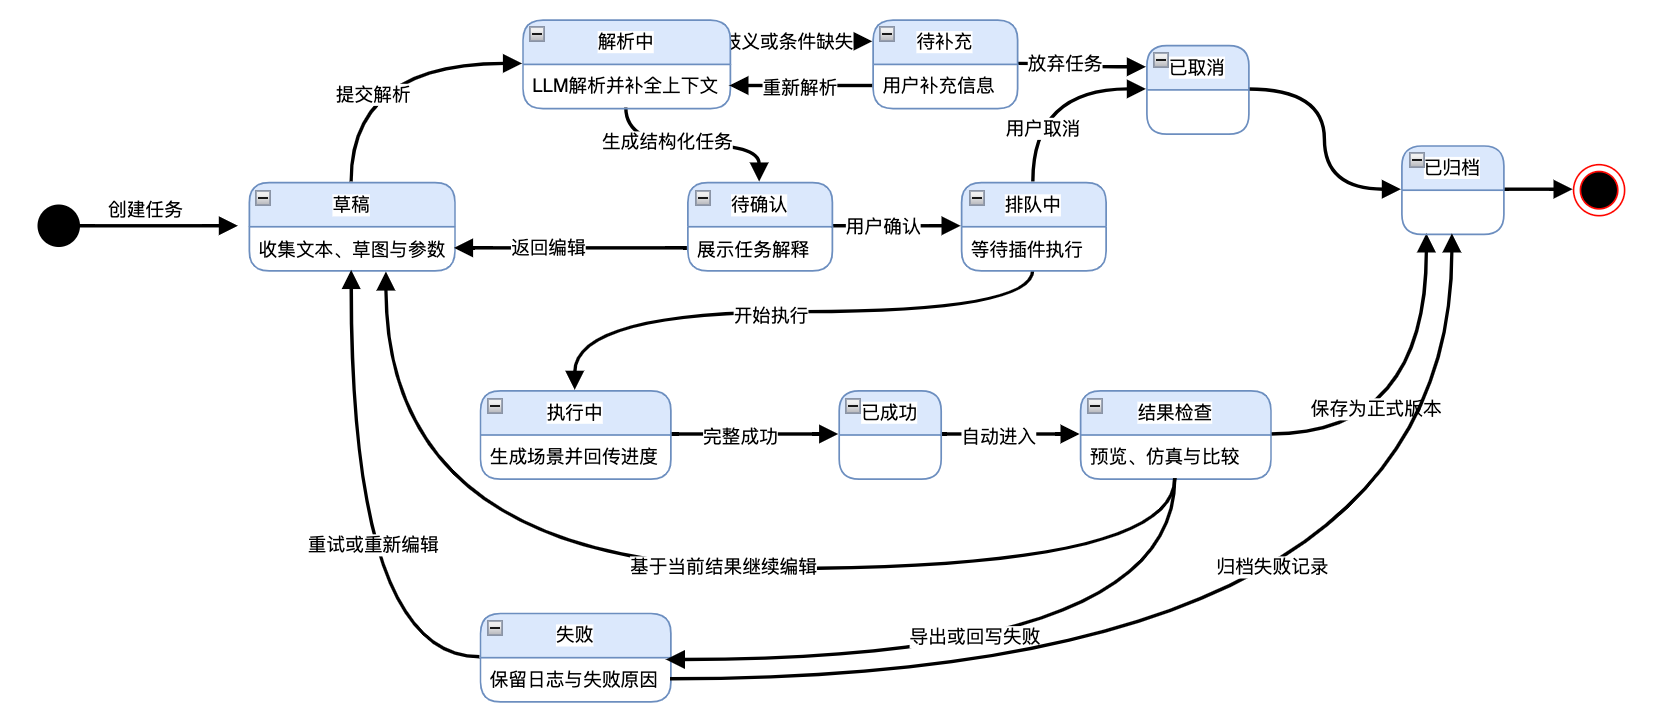
\includegraphics[width=\textwidth]{figures/06.png}
\caption{任务状态图}
\label{fig:oo_state}
\end{figure}

\subsection{构件图}
构件图~\ref{fig:oo_component} 给出了系统的软件构成单元及其依赖关系。主系统 UI 位于交互入口，任务调度服务位于核心控制位置，并分别依赖项目管理、权限、日志、LLM 接口适配和 Blender 插件适配等构件；Blender 插件适配器负责连接桌面端 Blender 插件；项目管理服务、日志服务和资源服务分别与数据库、文件存储和资产资源形成持久化依赖。

从构件分层上看，该图可以划分为交互层、服务层、执行层和基础设施层。交互层负责承接用户操作并展示结果；服务层负责项目管理、权限校验、任务调度、日志记录和资源访问；执行层负责连接 Blender 插件或外部模型服务；基础设施层负责数据库、文件和资产资源的持久化支撑。各层之间的依赖方向由上向下展开，避免交叉耦合。

该图的设计意义在于说明系统并不是以单进程方式实现所有功能，而是通过若干可替换、可扩展的构件协同工作。这样既便于隔离桌面端插件执行与服务端任务控制，也便于后续替换解析服务、调整存储实现或增加新的业务构件。

\begin{figure}[!htbp]
\centering
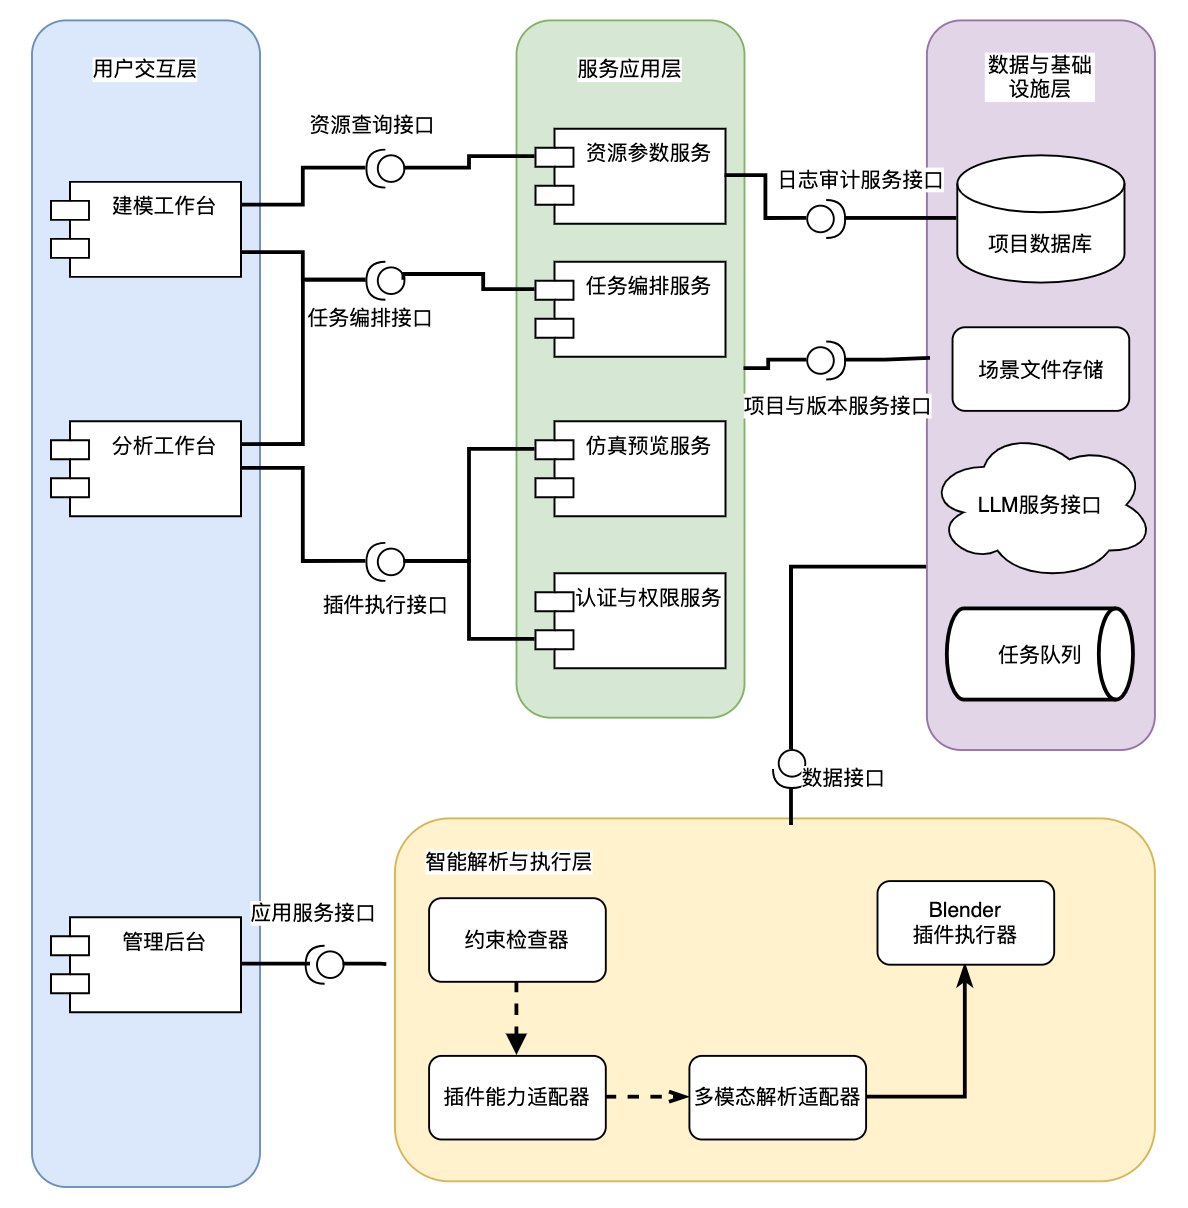
\includegraphics[width=\textwidth]{figures/07.png}
\caption{系统构件图}
\label{fig:oo_component}
\end{figure}

\subsection{部署图}
部署图~\ref{fig:oo_deployment} 描述了系统在运行环境中的节点划分与构件部署关系。用户工作站部署主系统前端界面、Blender 桌面端和城市生成插件；应用服务节点部署认证与权限服务、项目与版本服务、任务编排服务、资源参数服务、仿真预览服务和日志审计服务；模型服务节点部署 LLM 解析接口；数据与资源节点部署项目数据库、场景文件存储、资产资源库以及日志与备份目录。各节点之间通过登录鉴权、任务提交、解析请求、版本回写、资源读取和结果预览等通信链路相互连接，构成完整的运行环境。

从部署角色上看，用户工作站负责直接面向用户的交互与本地插件执行，应用服务节点负责业务控制与状态管理，模型服务节点负责解析能力输出，数据与资源节点负责持久化与资源供给。这样的部署划分使桌面执行环境、业务服务环境和模型推理环境相互分离，有利于分别扩展与维护。

从通信关系上看，前端界面既与应用服务节点交互，也通过任务编排服务间接驱动本地 Blender 插件；任务编排服务一方面向模型服务节点发起解析请求，另一方面向项目服务和日志服务写入上下文与执行结果；插件则直接访问场景文件存储和资产资源库完成本地生成与写盘。该图说明系统在运行层面采用“前端交互、本地执行、服务控制、集中存储”的协同方式。

\begin{figure}[!htbp]
\centering
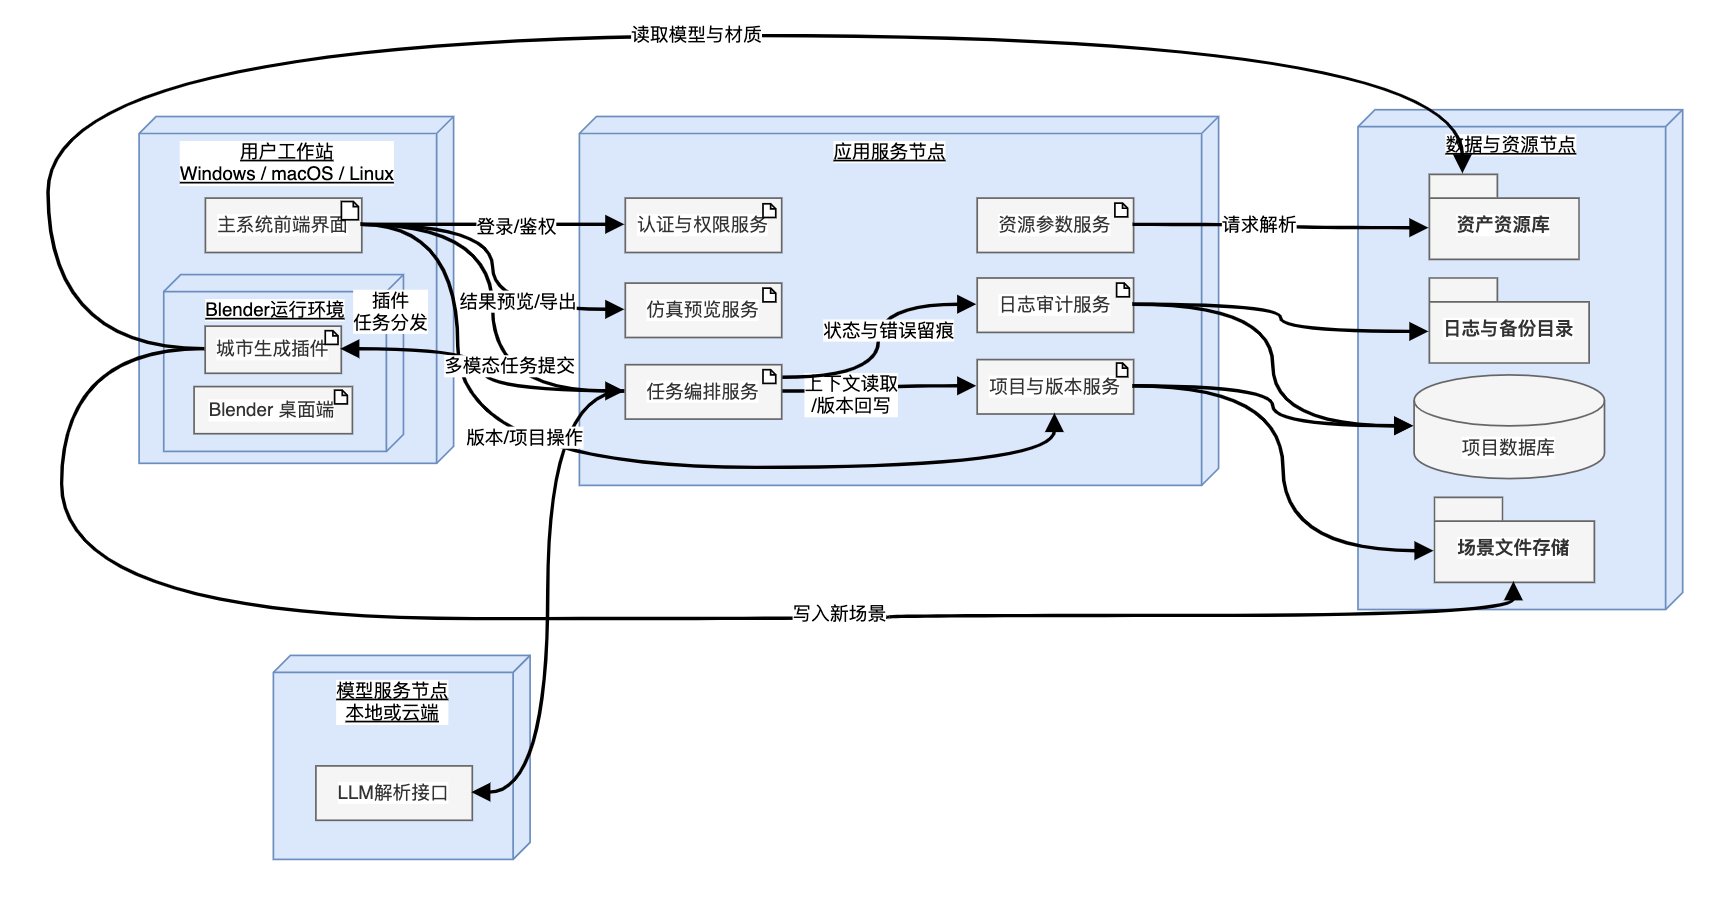
\includegraphics[width=\textwidth]{figures/08.png}
\caption{系统部署图}
\label{fig:oo_deployment}
\end{figure}

\subsection{统一命名与边界约定}
本章各类图在表达角度上各有侧重，但在命名和边界上保持一致。角色统一使用场景建模师、行业分析师和系统管理员；任务统一围绕 \texttt{Task}、\texttt{StructuredCommand}、\texttt{PluginJob} 和 \texttt{ExecutionResult} 组织；版本结果统一由 \texttt{SceneVersion} 承接；解析能力统一由 LLM 或解析执行服务承担；几何生成和场景落盘统一由 Blender 插件及其适配构件承担。这样的统一约定保证了各类图之间的语义连续性。
